\documentclass{article}\usepackage[]{graphicx}\usepackage[]{color}
%% maxwidth is the original width if it is less than linewidth
%% otherwise use linewidth (to make sure the graphics do not exceed the margin)
\makeatletter
\def\maxwidth{ %
  \ifdim\Gin@nat@width>\linewidth
    \linewidth
  \else
    \Gin@nat@width
  \fi
}
\makeatother

\definecolor{fgcolor}{rgb}{0.345, 0.345, 0.345}
\newcommand{\hlnum}[1]{\textcolor[rgb]{0.686,0.059,0.569}{#1}}%
\newcommand{\hlstr}[1]{\textcolor[rgb]{0.192,0.494,0.8}{#1}}%
\newcommand{\hlcom}[1]{\textcolor[rgb]{0.678,0.584,0.686}{\textit{#1}}}%
\newcommand{\hlopt}[1]{\textcolor[rgb]{0,0,0}{#1}}%
\newcommand{\hlstd}[1]{\textcolor[rgb]{0.345,0.345,0.345}{#1}}%
\newcommand{\hlkwa}[1]{\textcolor[rgb]{0.161,0.373,0.58}{\textbf{#1}}}%
\newcommand{\hlkwb}[1]{\textcolor[rgb]{0.69,0.353,0.396}{#1}}%
\newcommand{\hlkwc}[1]{\textcolor[rgb]{0.333,0.667,0.333}{#1}}%
\newcommand{\hlkwd}[1]{\textcolor[rgb]{0.737,0.353,0.396}{\textbf{#1}}}%

\usepackage{framed}
\makeatletter
\newenvironment{kframe}{%
 \def\at@end@of@kframe{}%
 \ifinner\ifhmode%
  \def\at@end@of@kframe{\end{minipage}}%
  \begin{minipage}{\columnwidth}%
 \fi\fi%
 \def\FrameCommand##1{\hskip\@totalleftmargin \hskip-\fboxsep
 \colorbox{shadecolor}{##1}\hskip-\fboxsep
     % There is no \\@totalrightmargin, so:
     \hskip-\linewidth \hskip-\@totalleftmargin \hskip\columnwidth}%
 \MakeFramed {\advance\hsize-\width
   \@totalleftmargin\z@ \linewidth\hsize
   \@setminipage}}%
 {\par\unskip\endMakeFramed%
 \at@end@of@kframe}
\makeatother

\definecolor{shadecolor}{rgb}{.97, .97, .97}
\definecolor{messagecolor}{rgb}{0, 0, 0}
\definecolor{warningcolor}{rgb}{1, 0, 1}
\definecolor{errorcolor}{rgb}{1, 0, 0}
\newenvironment{knitrout}{}{} % an empty environment to be redefined in TeX

\usepackage{alltt}
\usepackage[utf8]{inputenc}

\usepackage{xcolor}
\usepackage{listings}
\lstset{basicstyle=\ttfamily,
  showstringspaces=false,
  commentstyle=\color{red},
  keywordstyle=\color{blue}
}

\title{Problem Set 3}
\author{Alexander Brandt\\SID: 24092167}
\date{September 30 2015}
\IfFileExists{upquote.sty}{\usepackage{upquote}}{}
\begin{document}

\maketitle

\section{Debugging Reading}

I chose to read option ii) as I am a huge fan of the Software Carpentry Foundation, as well as Titus Brown's work in general.  My question was ``After reading the Software Carpentry Foundation's paper on 'Best Practices for Scientific Computing', I found myself wondering about section 9, which says 'Document design and purpose, not mechanics.'  When is code written in such a way that it is self-evident to an outside reader/developer?  What are the hallmarks of code written in this style?  I think the suggestion has good intentions, but often discerning the difficulty level associated block of code is challenging for developers.  One person's 'easy' is often another person's 'hard,' and so in this way applying the principle of "the onerous should always be on the author to convince his or her peers of that" seems to be to be a recipe for disaster in the hands of some very well-meaning scientific programmers that I know that have forgotten how difficult it can be to work within a certain language, leading to less commentary and comprehension, not more.  For example, would explaining a choice of data structure in a language (a dict vs. a list in Python, for example) be violating this principle?''


\section{An Analysis of the Presidental Election Debates}

My question is: 
\begin{knitrout}
\definecolor{shadecolor}{rgb}{0.969, 0.969, 0.969}\color{fgcolor}\begin{kframe}
\begin{alltt}
\hlkwd{library}\hlstd{(stringr)}
\hlkwd{library}\hlstd{(XML)}
\hlkwd{library}\hlstd{(curl)}

\hlstd{split_block} \hlkwb{<-} \hlkwa{function} \hlstd{(}\hlkwc{list_of_strings_solid}\hlstd{) \{}
  \hlstd{current_name} \hlkwb{=} \hlstr{""}
  \hlstd{current_block} \hlkwb{=} \hlstr{""}
  \hlstd{my_list} \hlkwb{=} \hlkwd{list}\hlstd{()}
  \hlstd{list_of_strings} \hlkwb{<-} \hlkwd{unlist}\hlstd{(}\hlkwd{strsplit}\hlstd{(list_of_strings_solid,}\hlstr{"\textbackslash{}n"}\hlstd{))}
  \hlcom{# XML example class notes -- different HTML features}
  \hlkwa{for} \hlstd{(i} \hlkwa{in} \hlnum{1}\hlopt{:}\hlkwd{length}\hlstd{(list_of_strings)) \{}
    \hlkwa{if} \hlstd{(((}\hlkwd{toupper}\hlstd{(list_of_strings[[i]])} \hlopt{==} \hlstd{list_of_strings[[i]])} \hlopt{&&}
         \hlopt{!}\hlkwd{grepl}\hlstd{(}\hlstr{"^\textbackslash{}\textbackslash{}([A-Z]+\textbackslash{}\textbackslash{})$"}\hlstd{,list_of_strings[[i]]))) \{}
      \hlcom{# This is a "caps line" which doesn't contain useful information about}
      \hlcom{# the text of the debate.  Mostly filler}
      \hlkwa{next}
    \hlstd{\}}
    \hlkwa{if} \hlstd{(}\hlkwd{grepl}\hlstd{(}\hlstr{"END"}\hlstd{,list_of_strings[[i]])) \{} \hlkwa{break} \hlstd{\}}
    \hlstd{name} \hlkwb{<-} \hlkwd{str_match}\hlstd{(list_of_strings[[i]],}\hlkwd{regex}\hlstd{(}\hlstr{"([A-Z]+):"}\hlstd{))[,}\hlnum{2}\hlstd{]}
    \hlkwa{if} \hlstd{((}\hlopt{!}\hlkwd{is.na}\hlstd{(name))} \hlopt{&&} \hlstd{name} \hlopt{!=} \hlstd{current_name) \{}
      \hlkwa{if} \hlstd{(current_name} \hlopt{!=} \hlstr{""}\hlstd{) \{}
        \hlstd{my_list[[current_name]]} \hlkwb{<-} \hlkwd{c}\hlstd{(my_list[[current_name]],}
        \hlkwd{str_replace_all}\hlstd{(current_block,}\hlkwd{paste}\hlstd{(current_name,}\hlstr{": "}\hlstd{,}\hlkwc{sep}\hlstd{=}\hlstr{""}\hlstd{),}
        \hlstr{""}\hlstd{))}
      \hlstd{\}}
      \hlstd{current_name} \hlkwb{<-} \hlstd{name}
      \hlstd{current_block} \hlkwb{<-} \hlstr{""}
      \hlcom{# ... and maybe add a new block to the list?}
    \hlstd{\}}
    \hlkwa{if} \hlstd{(}\hlkwd{length}\hlstd{(current_name)} \hlopt{!=} \hlnum{0}\hlstd{) \{}
      \hlkwa{if} \hlstd{(current_block} \hlopt{!=} \hlstr{""}\hlstd{) \{}
        \hlstd{current_block} \hlkwb{<-} \hlkwd{paste}\hlstd{(current_block,}
                               \hlstd{list_of_strings[[i]],} \hlkwc{sep}\hlstd{=}\hlstr{" "}\hlstd{)}
      \hlstd{\}}
      \hlkwa{else} \hlstd{\{}
        \hlstd{current_block} \hlkwb{<-} \hlstd{list_of_strings[[i]]}
      \hlstd{\}}
    \hlstd{\}}
  \hlstd{\}}
  \hlstd{my_list[[current_name]]} \hlkwb{<-} \hlkwd{c}\hlstd{(my_list[[current_name]],}
  \hlkwd{str_replace_all}\hlstd{(current_block,}
                  \hlkwd{paste}\hlstd{(current_name,}\hlstr{": "}\hlstd{,}\hlkwc{sep}\hlstd{=}\hlstr{""}\hlstd{),}\hlstr{""}\hlstd{))}
  \hlkwd{return}\hlstd{(my_list)}
\hlstd{\}}

\hlstd{create_debate_text} \hlkwb{<-} \hlkwa{function}\hlstd{(}\hlkwc{file_url}\hlstd{)}
\hlstd{\{}
  \hlstd{xml_handle} \hlkwb{<-} \hlkwd{htmlParse}\hlstd{(file_url)}
  \hlstd{v} \hlkwb{<-} \hlkwd{xpathSApply}\hlstd{(xml_handle,}
                   \hlstr{"//div[@id = 'content-sm']"}\hlstd{,xmlValue)}
  \hlstd{text_data} \hlkwb{<-} \hlkwd{lapply}\hlstd{(v,str_replace_all,}
                      \hlstr{"([A-Z]+:)"}\hlstd{,}\hlstr{"\textbackslash{}n\textbackslash{}n\textbackslash{}\textbackslash{}1"}\hlstd{)}
  \hlkwd{return}\hlstd{(text_data[[}\hlnum{1}\hlstd{]])}
\hlstd{\}}

\hlstd{debate_summary} \hlkwb{<-} \hlkwa{function}\hlstd{(}\hlkwc{file_url}\hlstd{)}
\hlstd{\{}
\hlstd{text_data} \hlkwb{<-} \hlkwd{create_debate_text}\hlstd{(file_url)}

\hlstd{events} \hlkwb{=} \hlkwd{list}\hlstd{()}
\hlstd{debate_blocks} \hlkwb{<-} \hlkwd{split_block}\hlstd{(text_data)}
\hlkwa{for} \hlstd{(n} \hlkwa{in} \hlkwd{names}\hlstd{(debate_blocks))}
\hlstd{\{}
   \hlstd{events[[n]]} \hlkwb{<-} \hlkwd{table}\hlstd{(}
     \hlkwd{str_extract_all}\hlstd{(}
       \hlkwd{paste}\hlstd{(debate_blocks[[n]],}\hlkwc{collapse}\hlstd{=}\hlstr{" "}\hlstd{)}
       \hlstd{,}\hlstr{"\textbackslash{}\textbackslash{}([A-Za-z]+\textbackslash{}\textbackslash{})"}\hlstd{))}
   \hlstd{debate_blocks[[n]]} \hlkwb{<-} \hlkwd{lapply}\hlstd{(debate_blocks[[n]],}
                                \hlstd{str_replace_all,}
                                \hlstr{"\textbackslash{}\textbackslash{}([A-Za-z]+\textbackslash{}\textbackslash{})"}\hlstd{,}\hlstr{""}\hlstd{)}
\hlstd{\}}

\hlstd{words} \hlkwb{=} \hlkwd{list}\hlstd{()}
\hlstd{sentence} \hlkwb{=} \hlkwd{list}\hlstd{()}
\hlstd{word_counts} \hlkwb{=} \hlkwd{list}\hlstd{()}
\hlstd{patterns} \hlkwb{=} \hlkwd{c}\hlstd{(}\hlstr{"I[^a-zA-Z]"}\hlstd{,} \hlstr{"we[^a-zA-Z]"}\hlstd{,} \hlstr{"America(n)?[^a-zA-Z]"}\hlstd{,}
             \hlstr{"democra(cy|tic)[^a-zA-Z]"}\hlstd{,} \hlstr{"republic[^a-zA-Z]"}\hlstd{,}
             \hlstr{"Democrat(ic)?[^a-zA-Z]"}\hlstd{,}\hlstr{"Republican[^a-zA-Z]"}\hlstd{,}
             \hlstr{"free(dom)?[^a-zA-Z]"}\hlstd{,} \hlstr{"war[^a-zA-Z]"}\hlstd{,}
             \hlstr{"God(?! bless)[^a-zA-Z]"}\hlstd{,}
             \hlstr{"(Jesus|Christ|Christian)[^a-zA-Z]"}\hlstd{,}
             \hlstr{"God bless[^a-zA-Z]"}\hlstd{)}
\hlkwa{for} \hlstd{(n} \hlkwa{in} \hlkwd{names}\hlstd{(debate_blocks))}
\hlstd{\{}
  \hlstd{to_analyze} \hlkwb{<-} \hlkwd{paste}\hlstd{(debate_blocks[[n]],}\hlkwc{collapse}\hlstd{=}\hlstr{" "}\hlstd{)}
  \hlkwa{for} \hlstd{(pattern} \hlkwa{in} \hlstd{patterns)}
  \hlstd{\{}
    \hlstd{word_counts[[n]][[pattern]]} \hlkwb{<-} \hlkwd{str_count}\hlstd{(to_analyze,pattern)}
  \hlstd{\}}
  \hlkwd{names}\hlstd{(word_counts[[n]])} \hlkwb{<-} \hlkwd{c}\hlstd{(}\hlstr{"I"}\hlstd{,}\hlstr{"we"}\hlstd{,}\hlstr{"America\{n\}"}\hlstd{,}
                               \hlstr{"democra\{cy,tic\}"}\hlstd{,}\hlstr{"republic"}\hlstd{,}
                               \hlstr{"Democrat\{,ic\}"}\hlstd{,}\hlstr{"Republican"}\hlstd{,}
                               \hlstr{"free\{,dom\}"}\hlstd{,}\hlstr{"war"}\hlstd{,}
                               \hlstr{"God (only)"}\hlstd{,}\hlstr{"God Bless"}\hlstd{,}
                               \hlstr{"\{Jesus, Christ, Christian\}"}\hlstd{)}
  \hlcom{# print(word_counts)}
  \hlstd{words[[n]]} \hlkwb{<-} \hlkwd{str_extract_all}\hlstd{(to_analyze,}
\hlstr{'(([:alpha:]+(\textbackslash{}'([:alpha:]+)?)?)|([:digit:]+(,([:digit:]+)?)?))'}\hlstd{)}
  \hlstd{sentence[[n]]} \hlkwb{<-} \hlkwd{str_extract_all}\hlstd{(to_analyze,}
\hlstr{"([:alpha:])(([:alpha:]|[:space:]|[:digit:]|\textbackslash{}'|,|-)*)(\textbackslash{}\textbackslash{}.|\textbackslash{}\textbackslash{}?|\textbackslash{}\textbackslash{}!)"}\hlstd{)}
  \hlkwd{print}\hlstd{(}\hlkwd{paste}\hlstd{(}\hlstr{"The average word length of "}\hlstd{,}
              \hlstd{n,}\hlstr{"'s speach is:"}\hlstd{,}\hlkwc{sep} \hlstd{=} \hlstr{""}\hlstd{))}
  \hlkwd{print}\hlstd{(}\hlkwd{mean}\hlstd{(}\hlkwd{rapply}\hlstd{(words[[n]],nchar)))}
  \hlkwd{print}\hlstd{(}\hlkwd{paste}\hlstd{(}\hlstr{"The number of characters (in the words) in "}\hlstd{,}
              \hlstd{n,}\hlstr{"'s speach is:"}\hlstd{,}\hlkwc{sep} \hlstd{=} \hlstr{""}\hlstd{))}
  \hlkwd{print}\hlstd{(}\hlkwd{sum}\hlstd{(}\hlkwd{rapply}\hlstd{(words[[n]],nchar)))}
  \hlkwd{print}\hlstd{(}\hlkwd{paste}\hlstd{(}\hlstr{"The number of words in "}\hlstd{, n,}\hlstr{"'s speach is:"}\hlstd{,}
              \hlkwc{sep} \hlstd{=} \hlstr{""}\hlstd{))}
  \hlkwd{print}\hlstd{(}\hlkwd{length}\hlstd{(}\hlkwd{unlist}\hlstd{(words[[n]])))}
  \hlkwd{print}\hlstd{(}\hlkwd{paste}\hlstd{(}\hlstr{"The buzzwords in "}\hlstd{, n,}\hlstr{"'s speach is:"}\hlstd{,}
              \hlkwc{sep} \hlstd{=} \hlstr{""}\hlstd{))}
  \hlkwd{print}\hlstd{(word_counts[[n]])}
  \hlkwd{print}\hlstd{(}\hlkwd{paste}\hlstd{(}\hlstr{"Event occurences in "}\hlstd{, n,}\hlstr{"'s speach is:"}\hlstd{,}
              \hlkwc{sep} \hlstd{=} \hlstr{""}\hlstd{))}
  \hlkwd{print}\hlstd{(events[[n]])}
\hlstd{\}}
\hlkwd{return}\hlstd{(debate_blocks)}
\hlstd{\}}

\hlstd{menu_url}\hlkwb{=}\hlstr{"http://www.debates.org/index.php?page=debate-transcripts"}
\hlstd{menu_xml_handle} \hlkwb{<-} \hlkwd{htmlParse}\hlstd{(menu_url)}
\hlstd{menu_nodes} \hlkwb{<-} \hlkwd{getNodeSet}\hlstd{(menu_xml_handle,}\hlstr{"//a[@href]"}\hlstd{)}
\hlstd{all_debate_links} \hlkwb{<-} \hlkwd{xpathSApply}\hlstd{(}
  \hlstd{menu_xml_handle,} \hlstr{"//a[@href]"}\hlstd{, xmlGetAttr,} \hlstr{'href'}\hlstd{)}
\hlstd{years} \hlkwb{<-} \hlkwd{c}\hlstd{(}\hlstr{"2012"}\hlstd{,}\hlstr{"2008"}\hlstd{,}\hlstr{"2004"}\hlstd{,}\hlstr{"2000"}\hlstd{,}\hlstr{"1996"}\hlstd{)}

\hlstd{year_reg} \hlkwb{<-} \hlkwd{paste}\hlstd{(}\hlstr{"("}\hlstd{,}
                  \hlkwd{paste}\hlstd{(}\hlkwd{paste}\hlstd{(years,}\hlkwc{collapse}\hlstd{=}\hlstr{"|"}\hlstd{),}
                        \hlstr{").+(First)"}\hlstd{,}
                        \hlkwc{sep}\hlstd{=}\hlstr{""}\hlstd{),}
                  \hlkwc{sep}\hlstd{=}\hlstr{""}\hlstd{)}

\hlstd{my_debate_links} \hlkwb{<-} \hlstd{all_debate_links[}\hlkwd{grepl}\hlstd{(}
  \hlstd{year_reg,}
  \hlkwd{sapply}\hlstd{(menu_nodes,xmlValue))]}
\hlstd{debate_blocks_list} \hlkwb{=} \hlkwd{list}\hlstd{()}
\hlstd{i} \hlkwb{<-} \hlnum{1}
\hlkwa{for} \hlstd{(year} \hlkwa{in} \hlstd{years)}
\hlstd{\{}
  \hlkwd{print}\hlstd{(}\hlkwd{paste}\hlstd{(}\hlstr{"The statistics for the first debate in"}\hlstd{,year,}\hlstr{"..."}\hlstd{))}
  \hlstd{debate_blocks_list[[year]]} \hlkwb{<-} \hlkwd{debate_summary}\hlstd{(my_debate_links[i])}
  \hlstd{i} \hlkwb{<-} \hlstd{i} \hlopt{+} \hlnum{1}
  \hlkwd{cat}\hlstd{(}\hlstr{"\textbackslash{}n\textbackslash{}n"}\hlstd{)}
\hlstd{\}}
\end{alltt}
\begin{verbatim}
## [1] "The statistics for the first debate in 2012 ..."
## [1] "The average word length of LEHRER's speach is:"
## [1] 4.399606
## [1] "The number of characters (in the words) in LEHRER's speach is:"
## [1] 6705
## [1] "The number of words in LEHRER's speach is:"
## [1] 1524
## [1] "The buzzwords in LEHRER's speach is:"
##                          I                         we 
##                         17                         20 
##                 America{n}            democra{cy,tic} 
##                          1                          0 
##                   republic              Democrat{,ic} 
##                          0                          1 
##                 Republican                 free{,dom} 
##                          1                          0 
##                        war                 God (only) 
##                          0                          0 
##                  God Bless {Jesus, Christ, Christian} 
##                          0                          0 
## [1] "Event occurences in LEHRER's speach is:"
## 
##  (APPLAUSE) (CROSSTALK) (inaudible) 
##           1          10           4 
## [1] "The average word length of OBAMA's speach is:"
## [1] 4.450814
## [1] "The number of characters (in the words) in OBAMA's speach is:"
## [1] 32531
## [1] "The number of words in OBAMA's speach is:"
## [1] 7309
## [1] "The buzzwords in OBAMA's speach is:"
##                          I                         we 
##                        119                        172 
##                 America{n}            democra{cy,tic} 
##                         18                          0 
##                   republic              Democrat{,ic} 
##                          0                          4 
##                 Republican                 free{,dom} 
##                          5                          3 
##                        war                 God (only) 
##                          2                          0 
##                  God Bless {Jesus, Christ, Christian} 
##                          0                          0 
## [1] "Event occurences in OBAMA's speach is:"
## 
## (CROSSTALK)  (LAUGHTER) 
##           4           3 
## [1] "The average word length of ROMNEY's speach is:"
## [1] 4.322593
## [1] "The number of characters (in the words) in ROMNEY's speach is:"
## [1] 33807
## [1] "The number of words in ROMNEY's speach is:"
## [1] 7821
## [1] "The buzzwords in ROMNEY's speach is:"
##                          I                         we 
##                        217                         94 
##                 America{n}            democra{cy,tic} 
##                         34                          1 
##                   republic              Democrat{,ic} 
##                          0                          4 
##                 Republican                 free{,dom} 
##                          5                          7 
##                        war                 God (only) 
##                          0                          0 
##                  God Bless {Jesus, Christ, Christian} 
##                          0                          0 
## [1] "Event occurences in ROMNEY's speach is:"
## 
## (CROSSTALK) (inaudible)  (LAUGHTER) 
##          11           2           1 
## 
## 
## [1] "The statistics for the first debate in 2008 ..."
## [1] "The average word length of LEHRER's speach is:"
## [1] 4.317448
## [1] "The number of characters (in the words) in LEHRER's speach is:"
## [1] 5617
## [1] "The number of words in LEHRER's speach is:"
## [1] 1301
## [1] "The buzzwords in LEHRER's speach is:"
##                          I                         we 
##                         14                          8 
##                 America{n}            democra{cy,tic} 
##                          0                          0 
##                   republic              Democrat{,ic} 
##                          0                          1 
##                 Republican                 free{,dom} 
##                          1                          0 
##                        war                 God (only) 
##                          0                          0 
##                  God Bless {Jesus, Christ, Christian} 
##                          0                          0 
## [1] "Event occurences in LEHRER's speach is:"
## 
##  (APPLAUSE) (CROSSTALK)  (LAUGHTER) 
##           1           4           1 
## [1] "The average word length of OBAMA's speach is:"
## [1] 4.368359
## [1] "The number of characters (in the words) in OBAMA's speach is:"
## [1] 33383
## [1] "The number of words in OBAMA's speach is:"
## [1] 7642
## [1] "The buzzwords in OBAMA's speach is:"
##                          I                         we 
##                        145                        220 
##                 America{n}            democra{cy,tic} 
##                         13                          1 
##                   republic              Democrat{,ic} 
##                          0                          0 
##                 Republican                 free{,dom} 
##                          2                          2 
##                        war                 God (only) 
##                         12                          0 
##                  God Bless {Jesus, Christ, Christian} 
##                          0                          0 
## [1] "Event occurences in OBAMA's speach is:"
## 
## (CROSSTALK)        (ph) 
##           3           1 
## [1] "The average word length of MCCAIN's speach is:"
## [1] 4.412685
## [1] "The number of characters (in the words) in MCCAIN's speach is:"
## [1] 31586
## [1] "The number of words in MCCAIN's speach is:"
## [1] 7158
## [1] "The buzzwords in MCCAIN's speach is:"
##                          I                         we 
##                        213                        141 
##                 America{n}            democra{cy,tic} 
##                         18                          1 
##                   republic              Democrat{,ic} 
##                          0                          1 
##                 Republican                 free{,dom} 
##                          2                          3 
##                        war                 God (only) 
##                          5                          0 
##                  God Bless {Jesus, Christ, Christian} 
##                          0                          0 
## [1] "Event occurences in MCCAIN's speach is:"
## 
## (CROSSTALK)  (LAUGHTER)        (ph)       (sic) 
##           1           1           1           1 
## 
## 
## [1] "The statistics for the first debate in 2004 ..."
## [1] "The average word length of LEHRER's speach is:"
## [1] 4.715942
## [1] "The number of characters (in the words) in LEHRER's speach is:"
## [1] 6508
## [1] "The number of words in LEHRER's speach is:"
## [1] 1380
## [1] "The buzzwords in LEHRER's speach is:"
##                          I                         we 
##                          9                          2 
##                 America{n}            democra{cy,tic} 
##                          2                          1 
##                   republic              Democrat{,ic} 
##                          0                          1 
##                 Republican                 free{,dom} 
##                          1                          0 
##                        war                 God (only) 
##                          3                          0 
##                  God Bless {Jesus, Christ, Christian} 
##                          0                          0 
## [1] "Event occurences in LEHRER's speach is:"
## 
##  (APPLAUSE) (CROSSTALK) 
##           2           1 
## [1] "The average word length of KERRY's speach is:"
## [1] 4.291059
## [1] "The number of characters (in the words) in KERRY's speach is:"
## [1] 30621
## [1] "The number of words in KERRY's speach is:"
## [1] 7136
## [1] "The buzzwords in KERRY's speach is:"
##                          I                         we 
##                        197                        114 
##                 America{n}            democra{cy,tic} 
##                         43                          2 
##                   republic              Democrat{,ic} 
##                          0                          0 
##                 Republican                 free{,dom} 
##                          1                          3 
##                        war                 God (only) 
##                         35                          0 
##                  God Bless {Jesus, Christ, Christian} 
##                          0                          1 
## [1] "Event occurences in KERRY's speach is:"
## 
## (LAUGHTER) 
##          2 
## [1] "The average word length of BUSH's speach is:"
## [1] 4.319169
## [1] "The number of characters (in the words) in BUSH's speach is:"
## [1] 27444
## [1] "The number of words in BUSH's speach is:"
## [1] 6354
## [1] "The buzzwords in BUSH's speach is:"
##                          I                         we 
##                        179                        122 
##                 America{n}            democra{cy,tic} 
##                         24                          4 
##                   republic              Democrat{,ic} 
##                          0                          0 
##                 Republican                 free{,dom} 
##                          0                         36 
##                        war                 God (only) 
##                         24                          1 
##                  God Bless {Jesus, Christ, Christian} 
##                          0                          0 
## [1] "Event occurences in BUSH's speach is:"
## 
## (LAUGHTER) 
##          1 
## 
## 
## [1] "The statistics for the first debate in 2000 ..."
## [1] "The average word length of MODERATOR's speach is:"
## [1] 4.558824
## [1] "The number of characters (in the words) in MODERATOR's speach is:"
## [1] 7750
## [1] "The number of words in MODERATOR's speach is:"
## [1] 1700
## [1] "The buzzwords in MODERATOR's speach is:"
##                          I                         we 
##                         14                         11 
##                 America{n}            democra{cy,tic} 
##                          0                          1 
##                   republic              Democrat{,ic} 
##                          0                          1 
##                 Republican                 free{,dom} 
##                          1                          0 
##                        war                 God (only) 
##                          0                          0 
##                  God Bless {Jesus, Christ, Christian} 
##                          0                          0 
## [1] "Event occurences in MODERATOR's speach is:"
## 
## (Applause) (APPLAUSE) 
##          1          1 
## [1] "The average word length of GORE's speach is:"
## [1] 4.339315
## [1] "The number of characters (in the words) in GORE's speach is:"
## [1] 31434
## [1] "The number of words in GORE's speach is:"
## [1] 7244
## [1] "The buzzwords in GORE's speach is:"
##                          I                         we 
##                        230                         72 
##                 America{n}            democra{cy,tic} 
##                         13                          1 
##                   republic              Democrat{,ic} 
##                          0                          1 
##                 Republican                 free{,dom} 
##                          1                          1 
##                        war                 God (only) 
##                          3                          0 
##                  God Bless {Jesus, Christ, Christian} 
##                          0                          0 
## [1] "Event occurences in GORE's speach is:"
## < table of extent 0 >
## [1] "The average word length of BUSH's speach is:"
## [1] 4.3035
## [1] "The number of characters (in the words) in BUSH's speach is:"
## [1] 32216
## [1] "The number of words in BUSH's speach is:"
## [1] 7486
## [1] "The buzzwords in BUSH's speach is:"
##                          I                         we 
##                        213                         83 
##                 America{n}            democra{cy,tic} 
##                         19                          1 
##                   republic              Democrat{,ic} 
##                          0                          2 
##                 Republican                 free{,dom} 
##                          1                          3 
##                        war                 God (only) 
##                          4                          0 
##                  God Bless {Jesus, Christ, Christian} 
##                          0                          0 
## [1] "Event occurences in BUSH's speach is:"
## < table of extent 0 >
## 
## 
## [1] "The statistics for the first debate in 1996 ..."
## [1] "The average word length of LEHRER's speach is:"
## [1] 4.691332
## [1] "The number of characters (in the words) in LEHRER's speach is:"
## [1] 4438
## [1] "The number of words in LEHRER's speach is:"
## [1] 946
## [1] "The buzzwords in LEHRER's speach is:"
##                          I                         we 
##                          6                          6 
##                 America{n}            democra{cy,tic} 
##                          0                          0 
##                   republic              Democrat{,ic} 
##                          0                          1 
##                 Republican                 free{,dom} 
##                          2                          0 
##                        war                 God (only) 
##                          0                          0 
##                  God Bless {Jesus, Christ, Christian} 
##                          0                          0 
## [1] "Event occurences in LEHRER's speach is:"
## < table of extent 0 >
## [1] "The average word length of CLINTON's speach is:"
## [1] 4.365762
## [1] "The number of characters (in the words) in CLINTON's speach is:"
## [1] 33612
## [1] "The number of words in CLINTON's speach is:"
## [1] 7699
## [1] "The buzzwords in CLINTON's speach is:"
##                          I                         we 
##                        243                        113 
##                 America{n}            democra{cy,tic} 
##                         34                          4 
##                   republic              Democrat{,ic} 
##                          0                          1 
##                 Republican                 free{,dom} 
##                          7                          8 
##                        war                 God (only) 
##                          2                          0 
##                  God Bless {Jesus, Christ, Christian} 
##                          0                          0 
## [1] "Event occurences in CLINTON's speach is:"
## < table of extent 0 >
## [1] "The average word length of DOLE's speach is:"
## [1] 4.308865
## [1] "The number of characters (in the words) in DOLE's speach is:"
## [1] 35044
## [1] "The number of words in DOLE's speach is:"
## [1] 8133
## [1] "The buzzwords in DOLE's speach is:"
##                          I                         we 
##                        276                        109 
##                 America{n}            democra{cy,tic} 
##                         42                          0 
##                   republic              Democrat{,ic} 
##                          0                          7 
##                 Republican                 free{,dom} 
##                         11                          1 
##                        war                 God (only) 
##                          2                          0 
##                  God Bless {Jesus, Christ, Christian} 
##                          0                          1 
## [1] "Event occurences in DOLE's speach is:"
## 
##    (ph) (staff) 
##       3       1
\end{verbatim}
\end{kframe}
\end{knitrout}

\section{Practice with S4 -- Illustrating a Random Walk}

\begin{knitrout}
\definecolor{shadecolor}{rgb}{0.969, 0.969, 0.969}\color{fgcolor}\begin{kframe}
\begin{alltt}
\hlstd{rw} \hlkwb{<-} \hlkwd{setClass}\hlstd{(}
  \hlstr{"rw"}\hlstd{,}
  \hlcom{# The basic slots associated with our class}
  \hlkwc{slots} \hlstd{=} \hlkwd{c}\hlstd{(}
    \hlkwc{start} \hlstd{=} \hlstr{"numeric"}\hlstd{,}
    \hlkwc{steps}   \hlstd{=} \hlstr{"numeric"}\hlstd{,}
    \hlkwc{trajectory_recording} \hlstd{=} \hlstr{"logical"}\hlstd{,}
    \hlkwc{.trajectory} \hlstd{=} \hlstr{"matrix"}\hlstd{),}

  \hlcom{# Now we declare our default values}
  \hlkwc{prototype}\hlstd{=}\hlkwd{list}\hlstd{(}
    \hlkwc{start} \hlstd{=} \hlkwd{c}\hlstd{(}\hlnum{0}\hlstd{,}\hlnum{0}\hlstd{),}
    \hlcom{#steps = 10,}
    \hlkwc{trajectory_recording} \hlstd{=} \hlnum{TRUE}
  \hlstd{),}
  \hlcom{# Look for things that might be amiss}
  \hlkwc{validity}\hlstd{=}\hlkwa{function}\hlstd{(}\hlkwc{object}\hlstd{)}
  \hlstd{\{}
    \hlcom{# REMEMBER TO ADD INTEGER CHECKS.}
    \hlkwa{if}\hlstd{(object}\hlopt{@}\hlkwc{steps}\hlopt{<}\hlnum{0}\hlstd{) \{}
      \hlkwd{return}\hlstd{(}\hlstr{"Please enter 
             a positive number of steps."}\hlstd{)}
    \hlstd{\}}
    \hlkwa{if}\hlstd{(}\hlkwd{as.integer}\hlstd{(object}\hlopt{@}\hlkwc{steps}\hlstd{)}\hlopt{!=}\hlstd{object}\hlopt{@}\hlkwc{steps}\hlstd{) \{}
      \hlkwd{return}\hlstd{(}\hlstr{"Please enter 
             an integer valued number of steps."}\hlstd{)}
    \hlstd{\}}
    \hlkwa{if}\hlstd{(}\hlkwd{length}\hlstd{(object}\hlopt{@}\hlkwc{start}\hlstd{)}\hlopt{!=}\hlnum{2}\hlstd{) \{}
      \hlkwd{return}\hlstd{(}\hlstr{"This program is
             only written for 2D (for now!)."}\hlstd{)}
    \hlstd{\}}
    \hlkwd{return}\hlstd{(}\hlnum{TRUE}\hlstd{)}
  \hlstd{\}}
\hlstd{)}


\hlcom{# Found "OOP in R" (http://practicalcomputing.org/node/80) to be very useful.}
\hlkwd{setGeneric}\hlstd{(}\hlstr{"start<-"}\hlstd{,} \hlkwa{function}\hlstd{(}\hlkwc{self}\hlstd{,} \hlkwc{value}\hlstd{)} \hlkwd{standardGeneric}\hlstd{(}\hlstr{"start<-"}\hlstd{))}
\end{alltt}
\begin{verbatim}
## [1] "start<-"
\end{verbatim}
\begin{alltt}
\hlkwd{setReplaceMethod}\hlstd{(}\hlstr{"start"}\hlstd{,}
  \hlstr{"rw"}\hlstd{,}
  \hlkwa{function}\hlstd{(}\hlkwc{self}\hlstd{,}\hlkwc{value}\hlstd{) \{}
  \hlstd{self}\hlopt{@}\hlkwc{start} \hlkwb{<-} \hlstd{value}
  \hlstd{self}
  \hlstd{\}}
\hlstd{)}
\end{alltt}
\begin{verbatim}
## [1] "start<-"
\end{verbatim}
\begin{alltt}
\hlkwd{setMethod}\hlstd{(}
  \hlkwc{f}\hlstd{=}\hlstr{"["}\hlstd{,}
  \hlkwc{signature}\hlstd{=}\hlstr{"rw"}\hlstd{,}
  \hlkwc{definition}\hlstd{=}\hlkwa{function}\hlstd{(}\hlkwc{x}\hlstd{,}\hlkwc{i}\hlstd{,}\hlkwc{drop}\hlstd{)\{}
    \hlstd{mypath}\hlkwb{=}\hlkwd{slot}\hlstd{(x,}\hlstr{".trajectory"}\hlstd{);}
    \hlstd{xs}\hlkwb{=}\hlkwd{sum}\hlstd{(mypath[}\hlnum{1}\hlopt{:}\hlstd{i,}\hlnum{1}\hlstd{]);}
    \hlstd{ys}\hlkwb{=}\hlkwd{sum}\hlstd{(mypath[}\hlnum{1}\hlopt{:}\hlstd{i,}\hlnum{2}\hlstd{]);}
    \hlkwd{return}\hlstd{(}\hlkwd{c}\hlstd{(x}\hlopt{@}\hlkwc{start}\hlstd{[}\hlnum{1}\hlstd{]}\hlopt{+}\hlstd{xs, x}\hlopt{@}\hlkwc{start}\hlstd{[}\hlnum{2}\hlstd{]}\hlopt{+}\hlstd{ys))}
  \hlstd{\}}
\hlstd{)}
\end{alltt}
\begin{verbatim}
## [1] "["
\end{verbatim}
\begin{alltt}
\hlkwd{setMethod}\hlstd{(}
  \hlkwc{f}\hlstd{=}\hlstr{"plot"}\hlstd{,}
  \hlkwc{signature}\hlstd{=}\hlstr{"rw"}\hlstd{,}
  \hlkwc{definition}\hlstd{=}\hlkwa{function}\hlstd{(}\hlkwc{x}\hlstd{)\{}
    \hlstd{mypath}\hlkwb{=}\hlkwd{slot}\hlstd{(x,}\hlstr{".trajectory"}\hlstd{);}
    \hlstd{xs}\hlkwb{=}\hlkwd{cumsum}\hlstd{(mypath[,}\hlnum{1}\hlstd{]);}
    \hlstd{ys}\hlkwb{=}\hlkwd{cumsum}\hlstd{(mypath[,}\hlnum{2}\hlstd{]);}
    \hlkwd{plot}\hlstd{(x}\hlopt{@}\hlkwc{start}\hlstd{[}\hlnum{2}\hlstd{]}\hlopt{+}\hlstd{ys,x}\hlopt{@}\hlkwc{start}\hlstd{[}\hlnum{1}\hlstd{]}\hlopt{+}\hlstd{xs,} \hlkwc{type}\hlstd{=}\hlstr{'o'}\hlstd{);}
  \hlstd{\}}
\hlstd{)}
\end{alltt}


{\ttfamily\noindent\itshape\color{messagecolor}{\#\# Creating a generic function for 'plot' from package 'graphics' in the global environment}}\begin{verbatim}
## [1] "plot"
\end{verbatim}
\begin{alltt}
\hlkwd{setMethod}\hlstd{(}
  \hlkwc{f}\hlstd{=}\hlstr{"print"}\hlstd{,}
  \hlkwc{signature}\hlstd{=}\hlstr{"rw"}\hlstd{,}
  \hlkwc{definition}\hlstd{=}\hlkwa{function}\hlstd{(}\hlkwc{x}\hlstd{)\{}
    \hlkwd{print}\hlstd{(}\hlstr{"Starting position:"}\hlstd{)}
    \hlkwd{print}\hlstd{(}\hlkwd{slot}\hlstd{(x,}\hlstr{"start"}\hlstd{))}
    \hlkwd{print}\hlstd{(}\hlstr{"After this many steps...:"}\hlstd{)}
    \hlkwd{print}\hlstd{(}\hlkwd{slot}\hlstd{(x,}\hlstr{"steps"}\hlstd{))}
    \hlkwd{print}\hlstd{(}\hlstr{"We arrive at:"}\hlstd{)}
    \hlkwd{print}\hlstd{(x[}\hlkwd{slot}\hlstd{(x,}\hlstr{"steps"}\hlstd{)])}
    \hlkwa{if} \hlstd{(}\hlkwd{slot}\hlstd{(x,}\hlstr{"trajectory_recording"}\hlstd{))}
    \hlstd{\{} \hlkwa{for} \hlstd{(i} \hlkwa{in} \hlnum{1}\hlopt{:}\hlkwd{slot}\hlstd{(x,}\hlstr{"steps"}\hlstd{)) \{}
        \hlkwd{print}\hlstd{(x[i]) \}\}}
  \hlstd{\}}
\hlstd{)}
\end{alltt}


{\ttfamily\noindent\itshape\color{messagecolor}{\#\# Creating a generic function for 'print' from package 'base' in the global environment}}\begin{verbatim}
## [1] "print"
\end{verbatim}
\begin{alltt}
\hlkwd{setGeneric}\hlstd{(}\hlstr{"simulate"}\hlstd{,}
           \hlkwa{function}\hlstd{(}\hlkwc{.Object}\hlstd{)\{}\hlkwd{standardGeneric}\hlstd{(}\hlstr{"simulate"}\hlstd{)\})}
\end{alltt}


{\ttfamily\noindent\itshape\color{messagecolor}{\#\# Creating a new generic function for 'simulate' in the global environment}}\begin{verbatim}
## [1] "simulate"
\end{verbatim}
\begin{alltt}
\hlkwd{setMethod}\hlstd{(}
  \hlkwc{f}\hlstd{=}\hlstr{"simulate"}\hlstd{,}
  \hlkwc{signature}\hlstd{=}\hlstr{"rw"}\hlstd{,}
  \hlkwc{definition}\hlstd{=}\hlkwa{function}\hlstd{(}\hlkwc{.Object}\hlstd{)\{}
    \hlkwd{slot}\hlstd{(.Object,}\hlstr{".trajectory"}\hlstd{)} \hlkwb{<-}
      \hlkwd{matrix}\hlstd{(}\hlkwd{c}\hlstd{(}\hlnum{0}\hlstd{,} \hlnum{1}\hlstd{,} \hlopt{-}\hlnum{1}\hlstd{,} \hlnum{0}\hlstd{,} \hlnum{1}\hlstd{,} \hlnum{0}\hlstd{,} \hlnum{0}\hlstd{,} \hlopt{-}\hlnum{1}\hlstd{),}
             \hlkwc{nrow}\hlstd{=}\hlnum{4}\hlstd{,}
             \hlkwc{ncol}\hlstd{=}\hlnum{2}\hlstd{)[}\hlkwd{sample}\hlstd{(}\hlnum{4}\hlstd{,}\hlkwc{size}\hlstd{=}\hlkwd{slot}\hlstd{(.Object,}\hlstr{"steps"}\hlstd{),}
             \hlkwc{replace}\hlstd{=}\hlnum{TRUE}\hlstd{),];}
    \hlkwd{return}\hlstd{(.Object)}
  \hlstd{\}}
\hlstd{)}
\end{alltt}
\begin{verbatim}
## [1] "simulate"
\end{verbatim}
\begin{alltt}
\hlcom{# Testing the replacement class}
\hlstd{my_walk} \hlkwb{<-} \hlkwd{new}\hlstd{(}\hlstr{"rw"}\hlstd{,} \hlkwc{start}\hlstd{=}\hlkwd{c}\hlstd{(}\hlnum{1}\hlstd{,}\hlnum{1}\hlstd{),}\hlkwc{steps}\hlstd{=}\hlnum{1000}\hlstd{,}\hlkwc{trajectory_recording}\hlstd{=}\hlnum{FALSE}\hlstd{)}
\hlcom{# To circumvent this, I would need to use the "assign" function, which}
\hlcom{# the S4 manual cautions against! }
\hlcom{# (https://cran.r-project.org/doc/contrib/Genolini-S4tutorialV0-5en.pdf)}
\hlstd{my_walk} \hlkwb{<-} \hlkwd{simulate}\hlstd{(my_walk)}
\hlstd{my_walk[}\hlnum{50}\hlstd{]}
\end{alltt}
\begin{verbatim}
## [1] 10  0
\end{verbatim}
\begin{alltt}
\hlkwd{plot}\hlstd{(my_walk)}
\end{alltt}
\end{kframe}
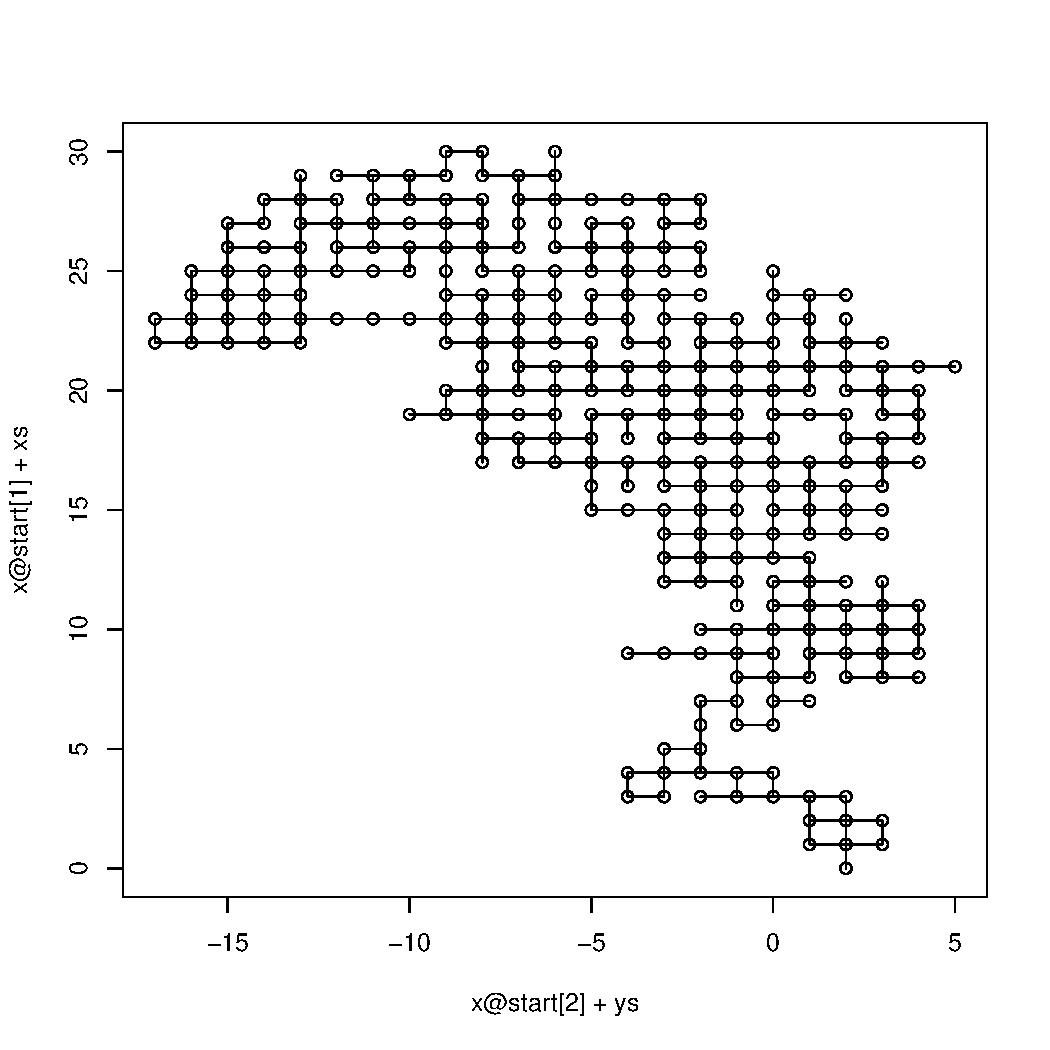
\includegraphics[width=\maxwidth]{figure/unnamed-chunk-2-1} 
\begin{kframe}\begin{alltt}
\hlkwd{start}\hlstd{(my_walk)}\hlkwb{<-}\hlkwd{c}\hlstd{(}\hlnum{100}\hlstd{,}\hlnum{100}\hlstd{)}
\hlkwd{plot}\hlstd{(my_walk)}
\end{alltt}
\end{kframe}
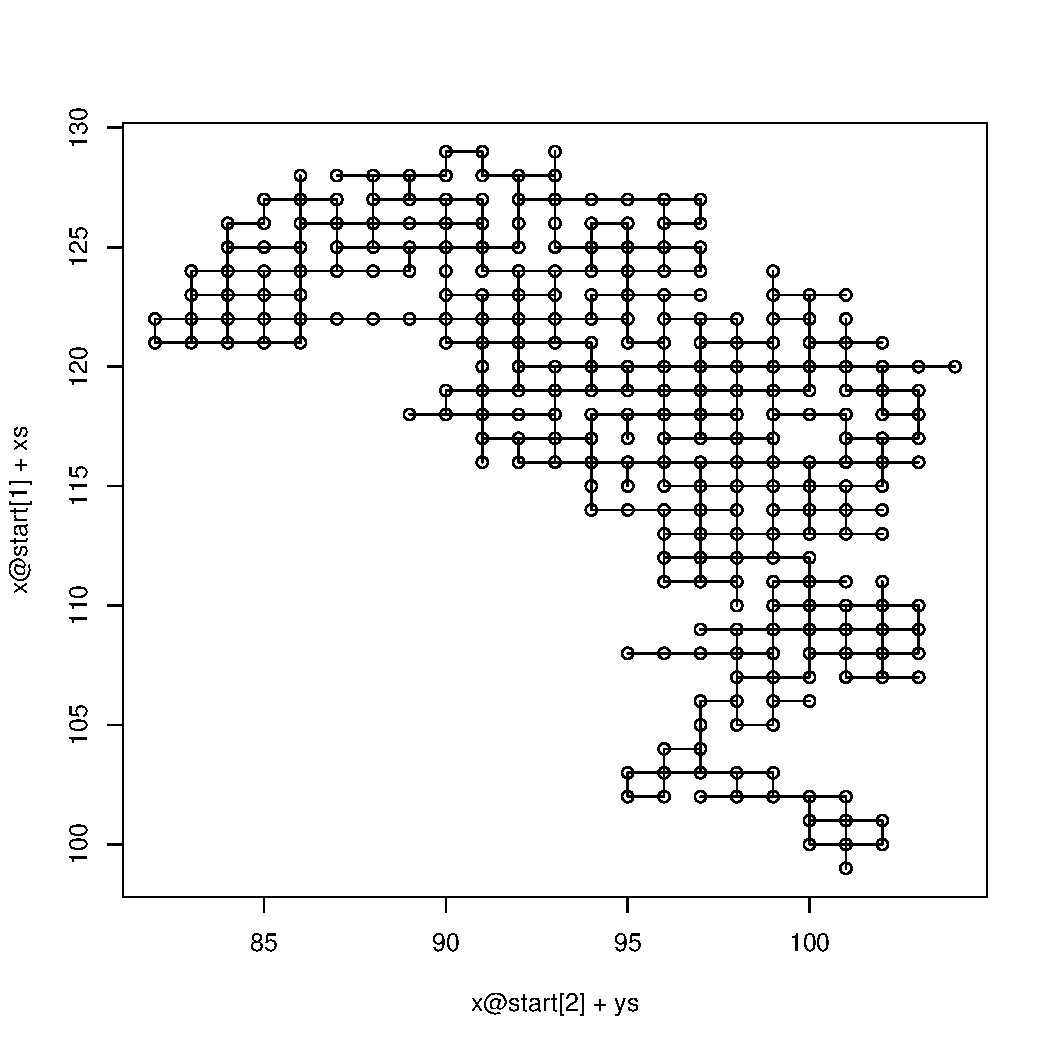
\includegraphics[width=\maxwidth]{figure/unnamed-chunk-2-2} 
\begin{kframe}\begin{alltt}
\hlkwd{print}\hlstd{(my_walk)}
\end{alltt}
\begin{verbatim}
## [1] "Starting position:"
## [1] 100 100
## [1] "After this many steps...:"
## [1] 1000
## [1] "We arrive at:"
## [1] 124  88
\end{verbatim}
\end{kframe}
\end{knitrout}

\end{document}
